\section{Люминесценция: виды люминесценции. Безызлучательные переходы, квантовый выход люминесценции. Фотолюминесценция жидкостей и твердых тел. Спектральный состав люминесценции. Правило Стокса. }

\subsection{Люминесценция: виды люминесценции}
\textbf{Люминесценция} - нетепловое излучение вещества (т.е. излучение сверх того, что при данной температуре излучает абсолютно черное тело). Природа явления заключается в следующем: электрону молекулы или атома неким способом сообщили избыточную энергию, он 'поднялся' на более высокий энергетический уровень, а затем 'вернулся', излучив при этом энергию в виде света. 


Виды люминесценции выделяются по способам подведения энергии к излучающим системам.

\textbf{Фотолюминесценция} — свечение под действием света (видимого и УФ-диапазона). Она, в свою очередь, делится на флуоресценцию (время жизни \(10^{-9}-10^{-6}\) с) и фосфоресценцию (\(10^{-3}-10\) с).


\textbf{Хемилюминесценция} — свечение, использующее энергию химических реакций. Примеры: свечение фосфора при медленном окислении, попы светлячков.


\textbf{Катодолюминесценция} — вызвана облучением быстрыми электронами (катодными лучами).


\textbf{Сонолюминесценция} — люминесценция, вызванная звуком высокой частоты. Примеры: вспышка света при схлопывании кавитационных пуырьков, рожденных в воде стоячей ультразвуковой волной.


\textbf{Триболюминесценция} — люминесценция, возникающая при растирании, раздавливании или раскалывании люминофоров. Триболюминесценция вызывается электрическими разрядами, происходящими между образовавшимися наэлектризованными частями — свет разряда вызывает фотолюминесценцию люминофора. Пример: разбивание рафинированного сахара.


\textbf{Электролюминесценция} - возникает при пропускании электрического тока через определённые типы люминофоров. Примеры: лампы дневного света.


\subsection{Безызлучательные переходы, квантовый выход люминесценции}


\textbf{Безызлучательные переходы} - 'переходы' на более высокие энергетические уровни без последующего 'возвращения' и излучения фотона. 

\textbf{Квантовый выход} - характеристика процесса люминесценции. Квантовый выход \(\phi\) определяется как:
\begin{equation}
    \phi = N_i / N_p,
\end{equation}
где \(N_i\) - среднее число излученных квантов,\(N_p\) - среднее число поглощенных квантов. Отличие этого показателя от единицы определяется как раз (в основном) наличием безызлучательных переходов.


{Энергетический выход} - так же характеристика люминесценции, только отношение средней излученной энергии к средней поглощенной энергии.

\subsection{Фотолюминесценция жидкостей и твердых тел}
В жидкостях и твердых телах фотолюминесценция часто "тушится" (легальный термин) при добавлении примесей, которые поглощают выделяющиеся кванты и перераспределяют их энергию в тепловое движение. Однако, при увеличении конценцтрации самого люминесцирующего вещества тоже наблюдается падение выхода флуоресценции (см. рис. \ref{landhui}).
\begin{figure}
    \centering
    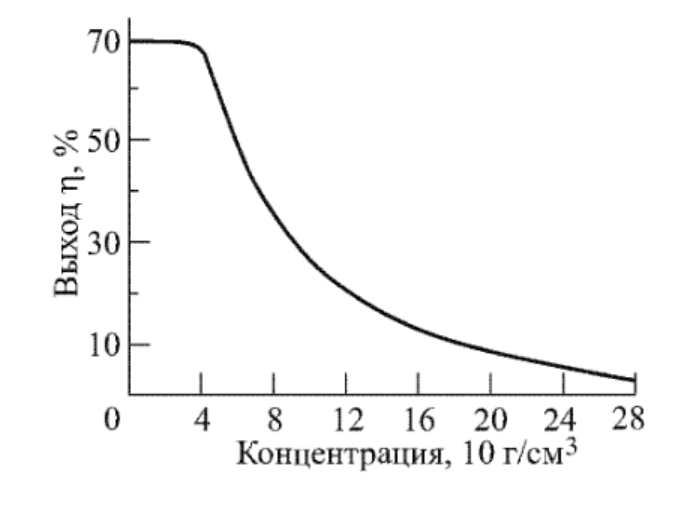
\includegraphics[scale = 0.5]{landhui.png}
    \caption{Зависимость выхода люминесценции от концентрации водного раствора флуорисцеинаю Иллюстрация из Ландсберга}
    \label{landhui}
\end{figure}

\subsection{Спектральный состав люминесценции}
Спектром люминесценции называют зависимость интенсивности люминесцентного излучения от длины волны испускаемого света. Наиболее простые — атомные спектры, в которых указанная выше зависимость определяется только электронным строением атома. Спектры молекул гораздо более сложные вследствие того, что в молекуле реализуются различные деформационные и валентные колебания. 

\subsection{Правило Стокса}
\textbf{Правило Стокса}: свет люминесценции имеет большую длину волны, чем поглощенный свет, вызвавший люминесценцию. (см. рис. \ref{lupaipupa}). Как и все, что названо словом "правило", иногда нарушается.
\begin{figure}[h!]
    \centering
    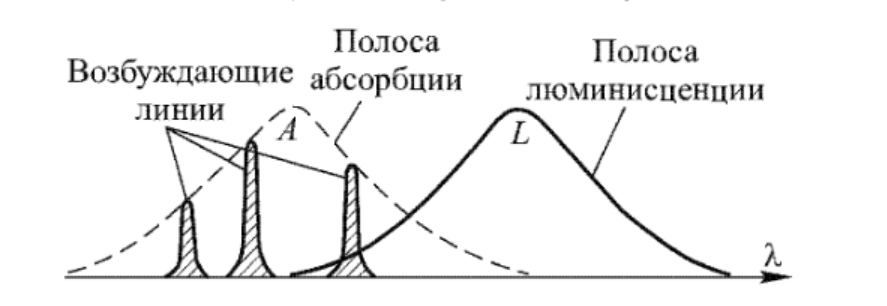
\includegraphics[scale = 0.5]{pupalupa.png}
    \caption{Схема, поясняющаяя правило Стокса. Максимум поглощения левее максимума испускания по шкале длин волн. Иллюстрация из Ландсберга}
    \label{lupaipupa}
\end{figure}
